\documentclass[a4paper, UKenglish, 11pt]{uiomaster}
\usepackage{lipsum}
\usepackage[subpreambles=true]{standalone}

% Explain EEG
% Explain how EEG sources can be modeled/simulated (include the first attempt done in 1949)
% Head models (New York Head Model)
% Maybe there should be an implementartion section ?

\begin{document}
\chapter{Results}
As mentioned in chapter 1, an important topic in EEG signal analysis is the inverse problem of going from measured EEG signals to localized equivalent current dipoles, so-called source localization. In this chapter we will present the training and performance of the neural networks presented in chapter 4. Section ... and ... deal with training of the simple feed forward neural network and presenting its results, while section ... will discuss how a convolution neural network can be used to obtain the same results. But first, we will take a look at the dataset being feed to the different networks.

\section{Simulation of EEG Signals}
The cortex matrix of the New York Head Model (NYHM) consists of 74382 points, which refer to the number of possible positions for localization of dipole sources. We will train the neural networks using a dataset of self-simulated EEG measurements that correspond to the electromagnetic fields generated by dipole sources. These sources will have randomly selected positions within the cortex matrix. However, to simplify the problem, the stengths of single dipoles (amplitude) are set to $10^7$ nA $\mu$ m. Moreover, in the cases of single dipole source localization, the direction of the dipole moment is always rotated so that it is normal to the cerebral cortex. In some cases this will result in a dipole moment pointing perpendicular to the skull (directed towards an EEG electorde), while in other cases, due to the structure of the cortex, the dipole moment will point back into the cortex (but eventually towards an EEG electorde). The reason for this is that the human cortex is strongly folded, and the contribution to the EEG signal from a neural population (dipole moment) will depend on whether a dipole is located in a sulcus or a gyrus (source: BookTVN).
\\
\\

\subsection{Effect of dipole location and orientation on EEG signals}
%The orientation of the cortical surface at a given location will, because of the sulci and gyri, affect how the local current dipoles will contribute to the EEG signal.
As shown by/ discussed in .... (source: BookTVN) EEG signals are relatively insensitive to small changes in the \emph{location} of neural current dipoles. Even though the intuitive thought might be that neurons in the upper cortical layers dominate the EEG due to the closer distance to the EEG electrode compared to neurons in the lower cortical layers, such differences in location acutually does not make conciderable differences. This finding can be explained by fact that the low conductivity of the skull generates a certain spatial low-pass filtering, that .... .
% Maybe what is meant here is that we therefore only consider the outer corical surface

\begin{figure}[!htb]
    \centering
    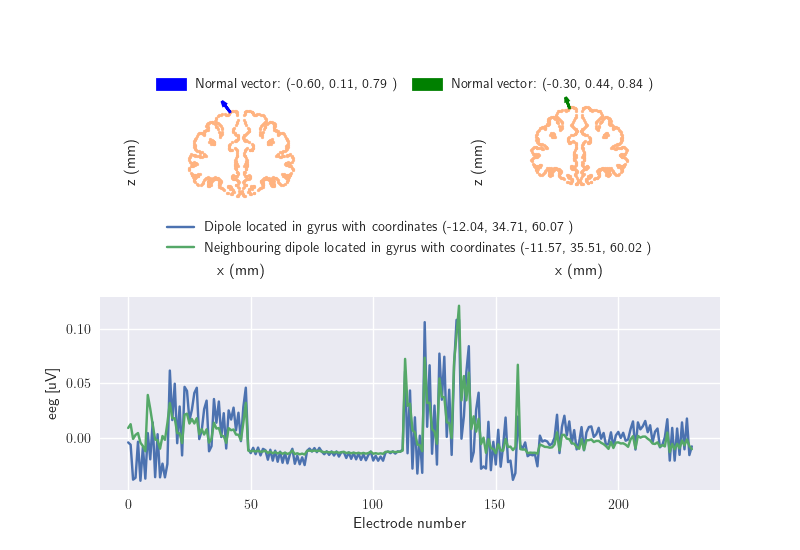
\includegraphics[width=\linewidth]{figures/neighbour_dipoles.png}
    \caption{EEG signal for neighbouring dipoles.}
    \label{fig:neighbour_dipoles}
\end{figure}

However, in order to decribe the effect of the \emph{orientation} of the dipoles relative to the EEG electrodes, we have in Figure \ref{fig:gyrus_and_sulcus_EEG} provided the EEG signals from two manually chosen dipole locations in the New York head model. The two dipoles illusrated are located in a gyrus and in a sulcus, both providing a different EEG outcome. In general, the EEG signal contribution from a single current dipole is maximized if the dipole is located in a gyrus, perpendicular oriented. Such a case is depiced in Figure \ref{fig:gyrus_and_sulcus_EEG}B. However, if we place a dipole in a sulcus, again with perpendicular orientation, we can observe a substantial EEG contribution, but in contrast to the dipole in the gyrus we notice a more dipolar pattern \ref{fig:gyrus_and_sulcus_EEG}C.

\begin{figure}[!htb]
    \centering
    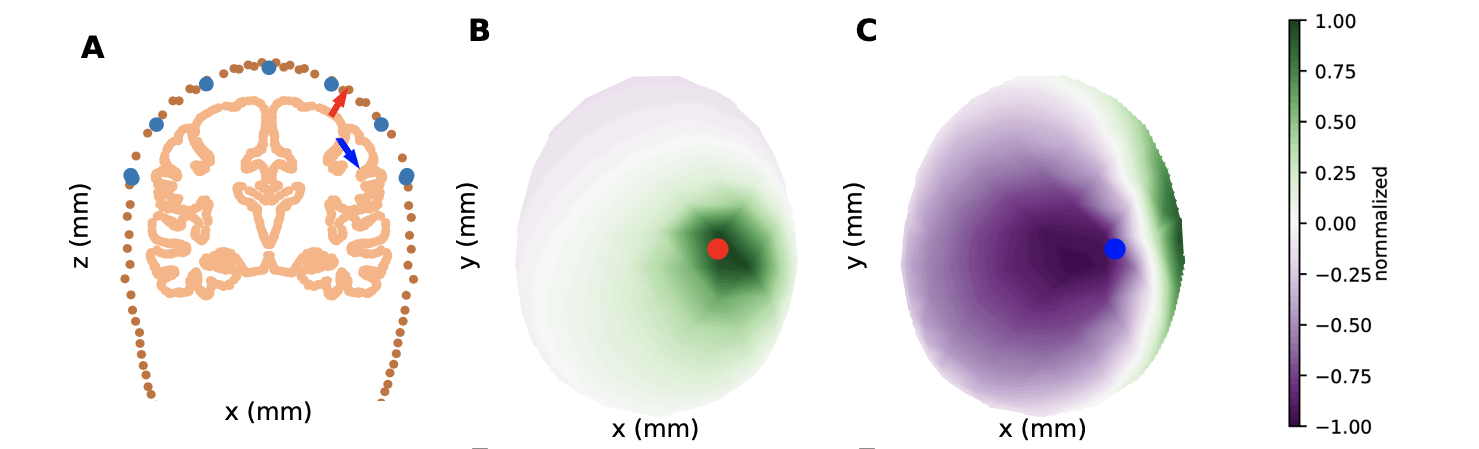
\includegraphics[width=\linewidth]{figures/gyrus_and_sulcus_EEG.png}
    \caption{A: Two manually chosen dipole locations in the New York head model, located in a gyrus (red) and a sulcus (blue). The head model is seen from the side (x, z-plane). EEG electrode locations close to the chosen cross section plane are marked in light blue. The available dipole locations close to the cortical cross section effectively draw an outline of the cortical sheet, and are marked in pink. The current dipole moment was in all cases $10^7$ nA$\mu$m. B: Interpolated color plot of EEG signal from the dipole in gyrus, seen from the top (x, y-plane). The plotted EEG signal is normalized but the maximal value was 1.1 $\mu$V. C: Interpolated color plot of EEG signal from the dipole in sulcus. The plotted EEG signal is normalized but the maximal value was 0.7 $\mu$V. (source: BookTVN)}
    \label{fig:gyrus_and_sulcus_EEG}
\end{figure}
\\
\\


\subsection{Noise}
As for all experimental data, real EEG recordings contain noise. Artifacts are signals recorded by EEG but with a origin different from those generated by human brain activity. As some artifact may mimic true epileptiform abnormalities or seizures, awereness of artifacts and methods for distinguishing such signals from brain waves is highly important (\url{https://link.springer.com/chapter/10.1007/978-3-030-03511-2_8}).

There are two different dypes of artifacts, classified according to their origin. Physiological artifacts originate from the patient itself, where the most usual ones are ocular activity, muscle activity, cardiac activity, perspiration and respiration. Technical artifacts, on the other hand, is generated from the environment of the patient, such as cable and body movements or electromagnetic interferences. (\url{https://www.bitbrain.com/blog/eeg-artifacts}).

Filtering techniques are usually utilized in order to remove artifact from EEG before analyzation of the recordings. But, when it comes to the simulated EEG data of ours, we are in no need to remove such noise, as there simply is none. The simulated EEG data can be understood as already filtered data that has undergone preprocessing steps, to ensure a high signal-to-noise ratio (\url{https://en.wikipedia.org/wiki/Signal-to-noise-ratio}). Moreover we understand the simulated data as an averaged measure of the typical EEG time series. However, in order to avoid overfiting and for other tecnical detailes, we do need to ass noise to tha data before feeding it to the neural network. Therefore, to the final dataset of ours we add normally distributed noise of 10 $\%$, with mean .... and standard deviation ... .


\section{Localizing Single Dipole Sources}

\subsection{The dataset}
The data set used to train a simple feed forward neural network consists of 10 000 rows, where each row corresponds to one sample, or let us say - one patient. Within the data set we have 231 columns, also referred to as features, representing the EEG measure at every recording electrode. Thus, we are left with a design matrix of size 10 000 x 231.

An example of how the input EEG data may look like for one sample (before adding noise) is provided in figure \ref{fig:eeg_field_1_dipole_example}. The figure illustrates the EEG result from a sample containing a single current dipole source at a random position within the celebral cortex. As also can be seen from the characteristic dipolar pattern, the dipole is located in a sulcus. The EEG measure is seen from both sides (x-, z-plane and y-, z-plane) and above (the x-, y-plane). EEG electrode locations are presented as filled circels, where the color of the fill represents the amplitude of the measured signal for the given electrode. The position of the current dipole moment is marked with a yellow star. As can be read off from the figure, the EEG signals, for this given sample, range from between -1 to 1 $\mu V$.

% How it looks when we add noise.
% Maybe add arrow and dipole direction??
\begin{figure}[!htb]
    \centering
    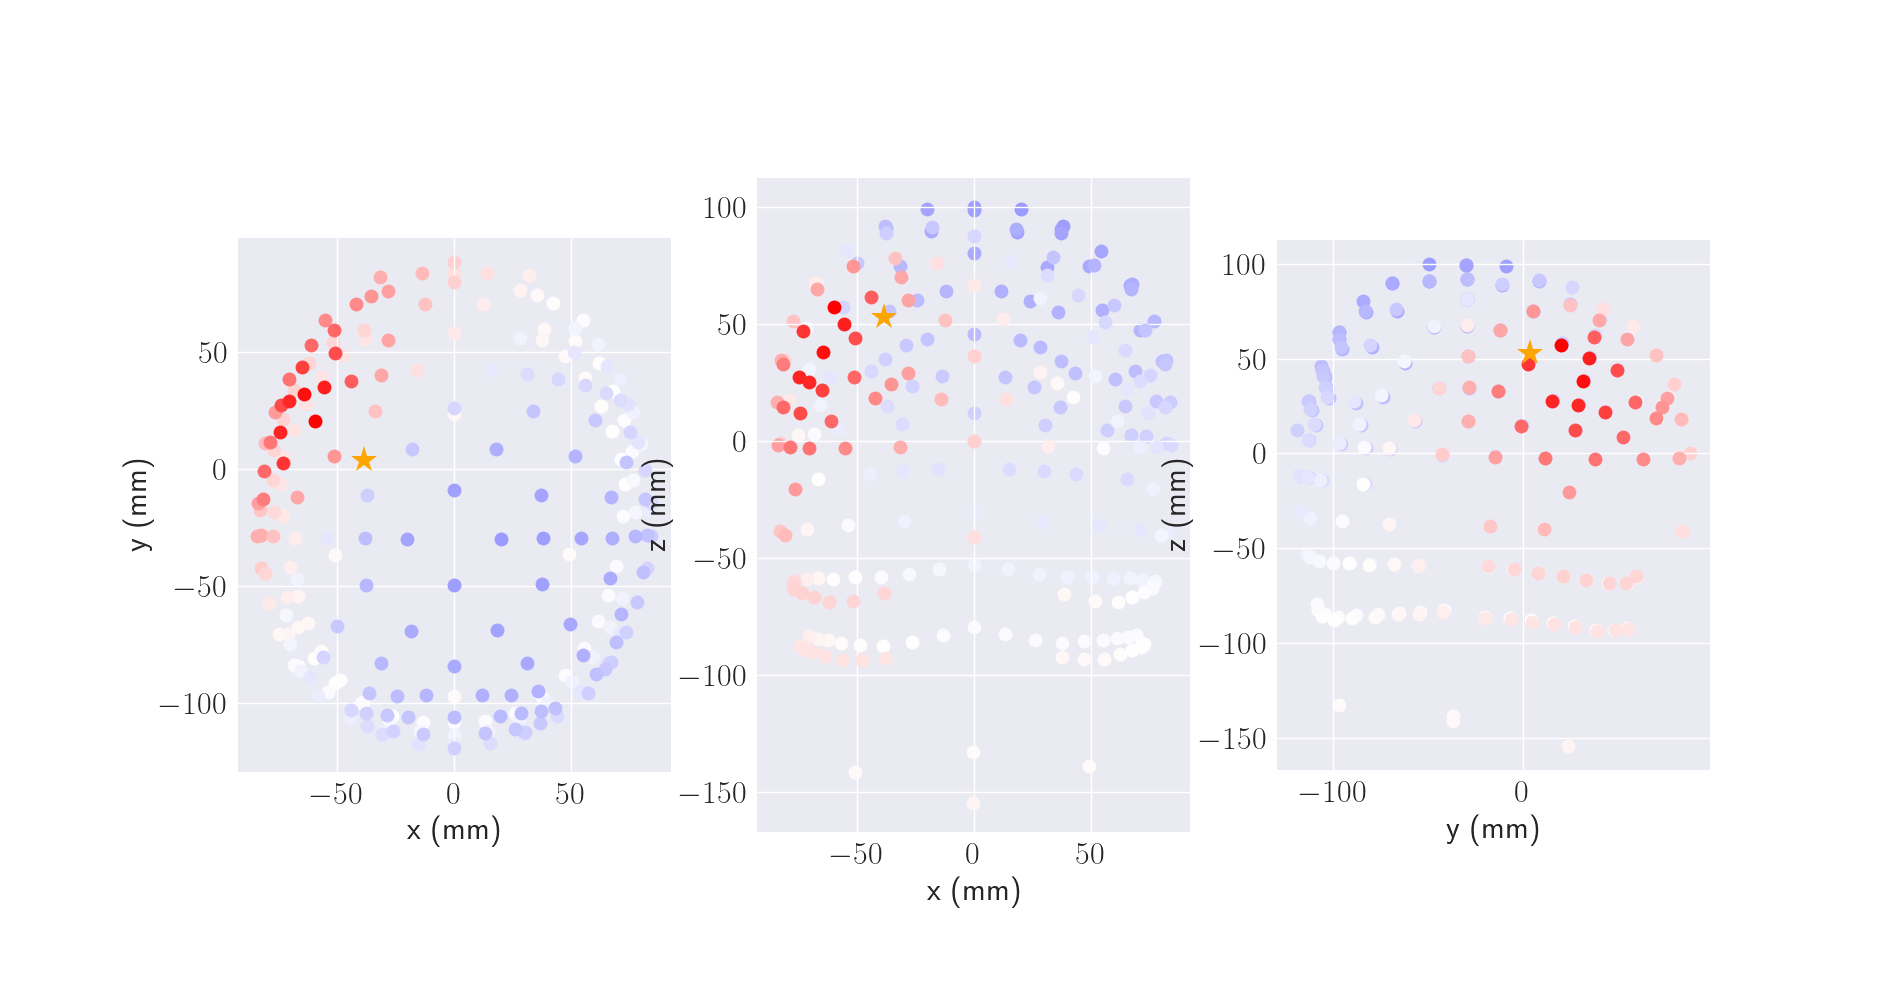
\includegraphics[width=\linewidth]{../Code/plots/finals/eeg_field_1_1.png}
    \caption{EEG for a sample containing one single current dipole source at a random position within the celebral cortex. The EEG measure is seen from both sides (x-, z-plane and y-, z-plane) and above (the x-, y-plane). EEG electrode locations are presented as filled circels, where the color of the fill represents the amplitude of the measured signal for the given electrode. The position of the current dipole moment is marked with a yellow star.}
    \label{fig:eeg_field_1_dipole_example}
\end{figure}

\subsection{Validation accuracy}
In Figure \ref{fig:single_dipole_accuracy} we have provided the validation accuray, using mean squared error (MSE) and the coefficient of determination (R2-score).

The expression for MSE when predicting the x-, y- and z-coordinate, goes as follows:

\begin{equation}
MSE(\hat{y},\hat{\tilde{y}}) &= \frac{1}{n}
\sum_{i=1}^{n}(y_i-\tilde{y}_i)^2 \\
&= \frac{1}{3}\sum_{i=1}^{3}((x-\tilde{x})^2 + (y-\tilde{y})^2 + (z-\tilde{z})^2 )
\label{eq:MSE}
\end{equation}

The coefficient of determination is given as follows:
\begin{equation}
R^2(\hat{y}, \tilde{\hat{y}}) = 1 - \frac{\sum_{i=0}^{n - 1} (y_i - \tilde{y}_i)^2}{\sum_{i=0}^{n - 1} (y_i - \bar{y})^2},
\label{eq:R2}
\end{equation}

Where the mean value of $y_i$ is defined by $\bar{y}$:

\begin{equation*}
\bar{y} =  \frac{1}{n} \sum_{i=0}^{n - 1} y_i.
\label{eq:ybar}
\end{equation*}


\begin{figure}[!htb]
    \centering
    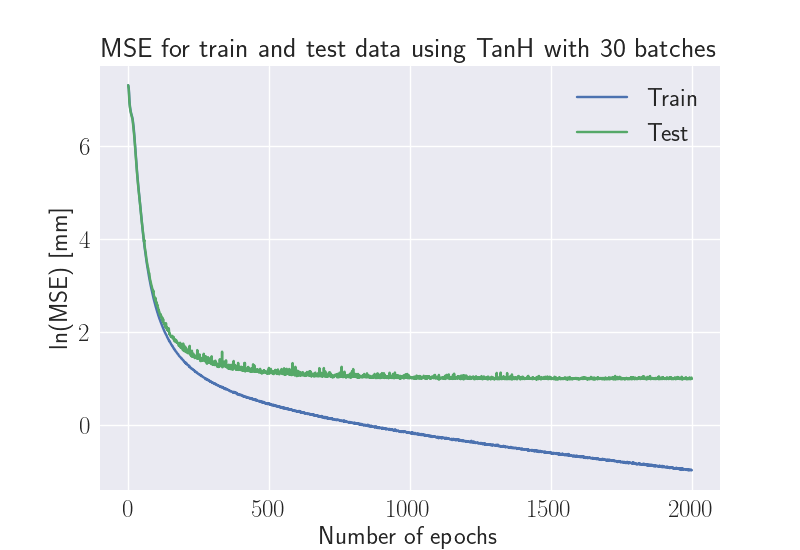
\includegraphics[width=\linewidth]{../Code/plots/finals/MSE_NN_1_10000_TanH_30_2000.png}
    \caption{The validation accuracy for the simple Feed Forward Neural Network with 10 000 samples with tanh activation function. }
    \label{fig:single_dipole_accuracy}
\end{figure}

\begin{figure}[!htb]
    \centering
    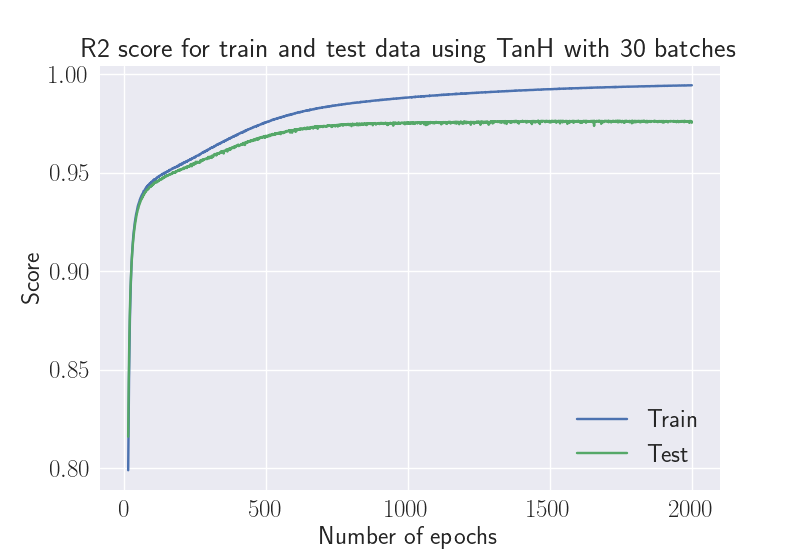
\includegraphics[width=\linewidth]{../Code/plots/finals/R2_NN_1_10000_l1_TanH_30_2000.png}
    \caption{The R2 score for the simple Feed Forward Neural Network with 10 000 samples with tanh activation function. }
    \label{fig:single_dipole_R2}
\end{figure}

\begin{figure}[!htb]
    \centering
    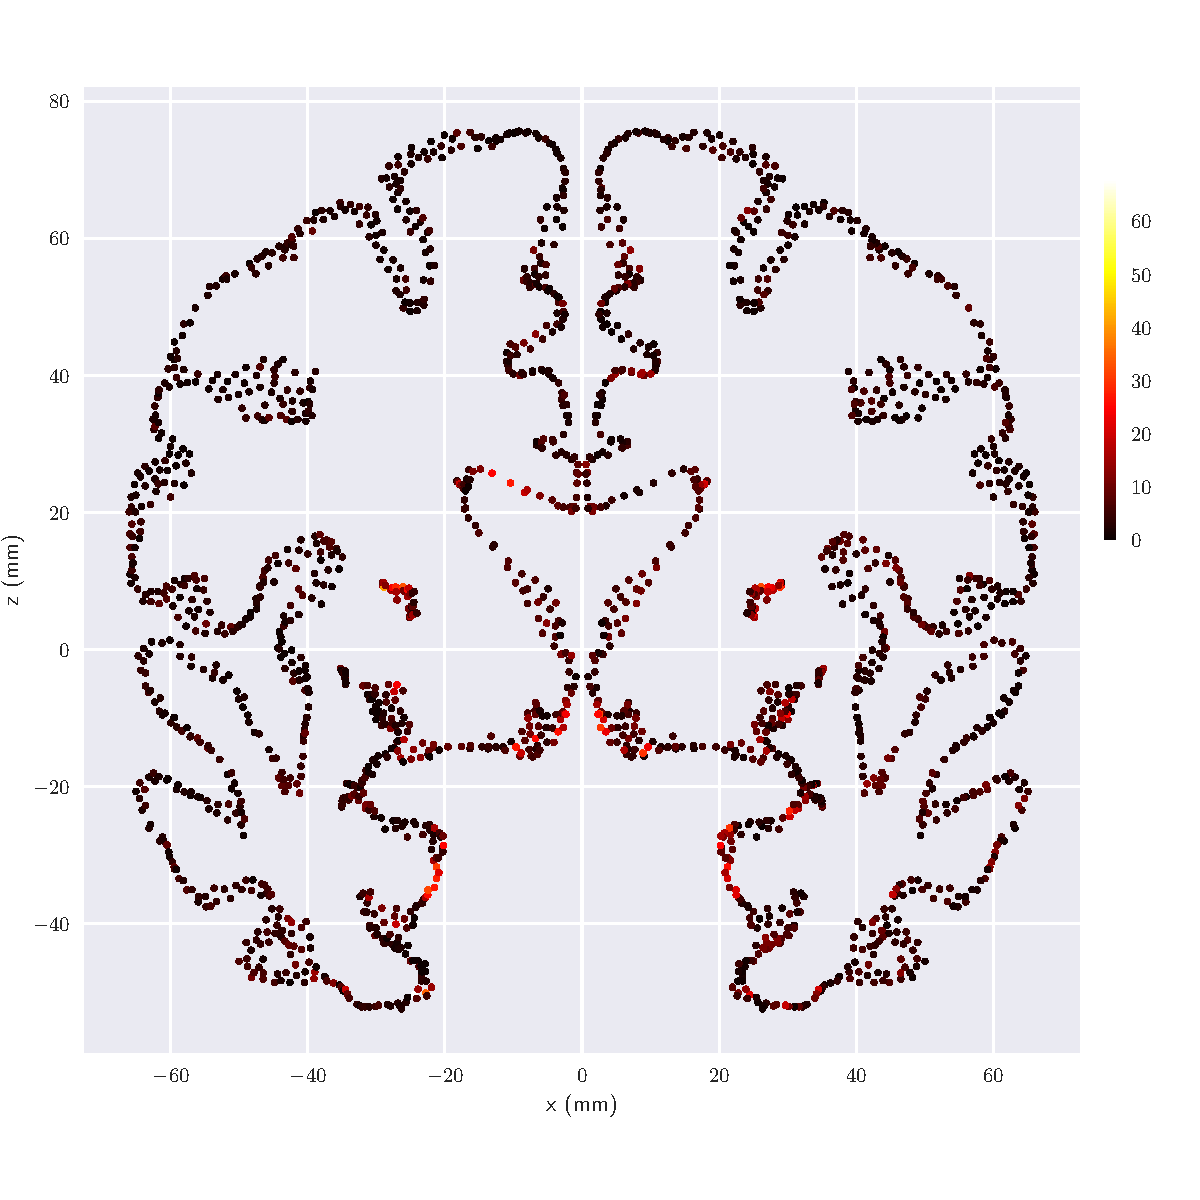
\includegraphics[width=\linewidth]{../Code/plots/finals/mse_y_plane.pdf}
    \caption{The mean squared error of the location accuracy (NN) at different dipole locations
    in the y cross section, for the simple Feed Forward Neural Network.}
    \label{fig:single_dipole_accuracy_plane}
\end{figure}



% \begin{figure}[!htb]
%     \centering
%     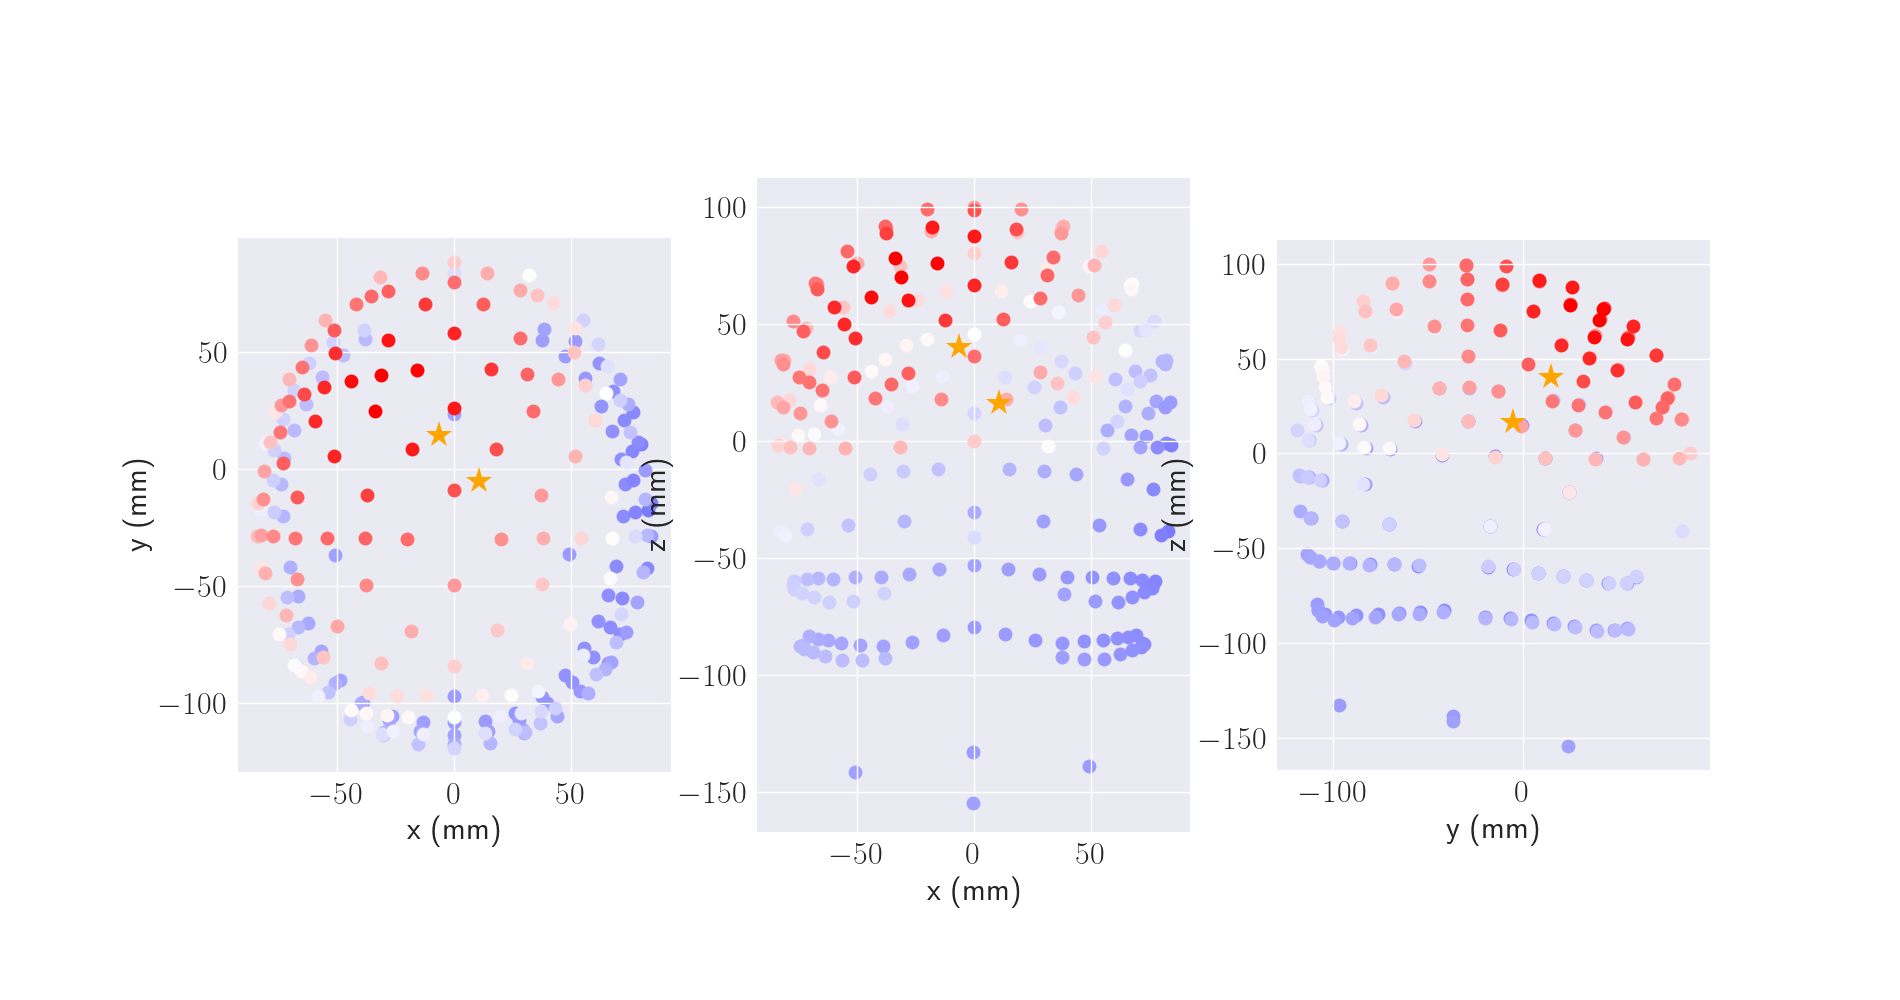
\includegraphics[width=\linewidth]{../Code/plots/finals/eeg_field_2_2.png}
%     \caption{Example 2 dipoles. }
%     \label{fig:eeg_field_2_dipole_example}
% \end{figure}



% \begin{figure}[!htb]
%     \centering
%     \includegraphics[width=\linewidth]{../Code/plots/NN/MSE_NN_noise_TanH_100_3000.png}
%     \caption{The validation accuracy for simple Feed Forward Neural Network with 10 000 samples with tanh activation function and 10$\%$ noise added to the data. }
%     \label{fig:single_dipole_accuracy}
% \end{figure}




\section{Convolution Neural Network Approach for localizing single dipole sources}

Some results for the prediction of location for single current dipoles.


\begin{figure}[!htb]
\centering
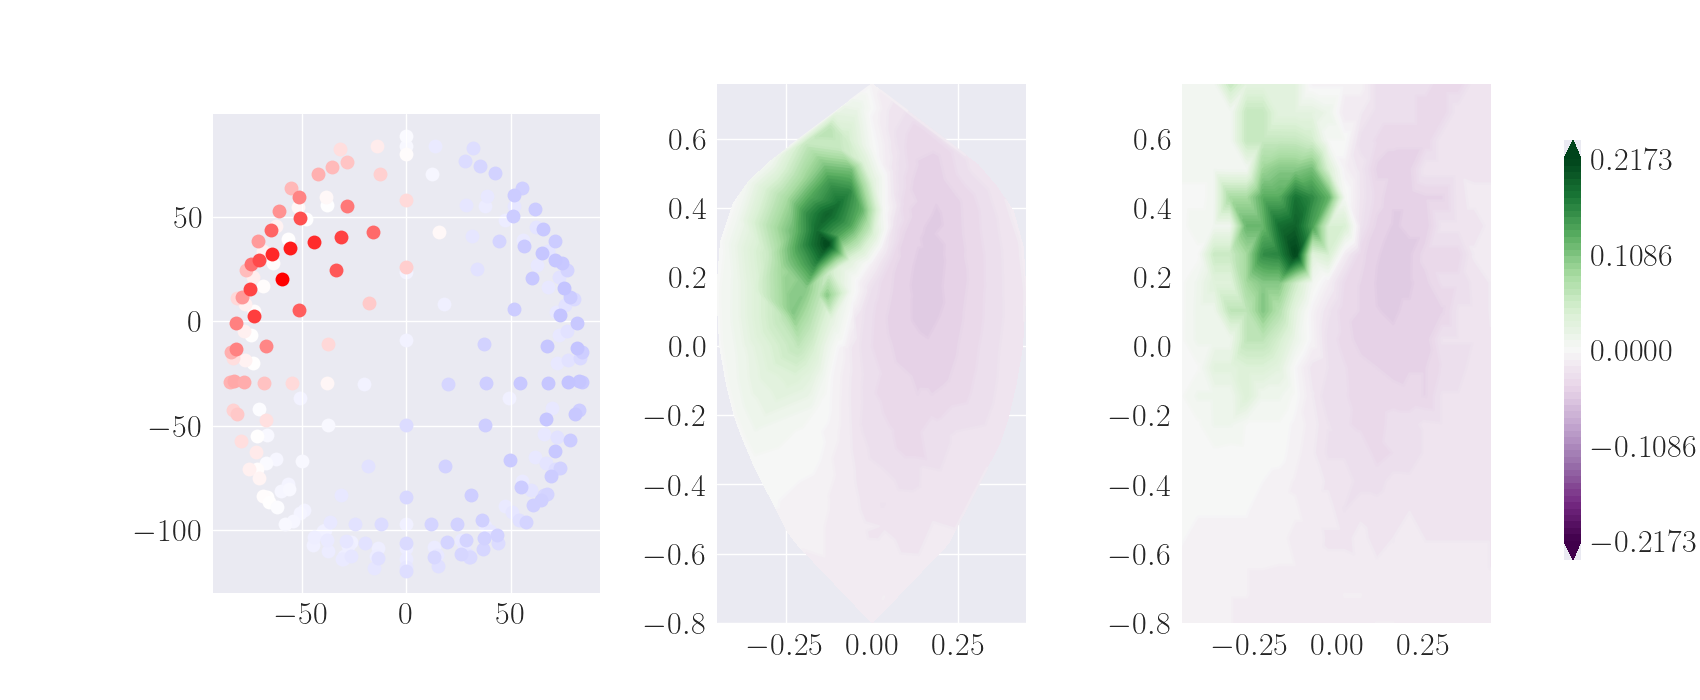
\includegraphics[width=\linewidth]{../Code/plots/finals/new_eeg_dipole_pos_0.png}
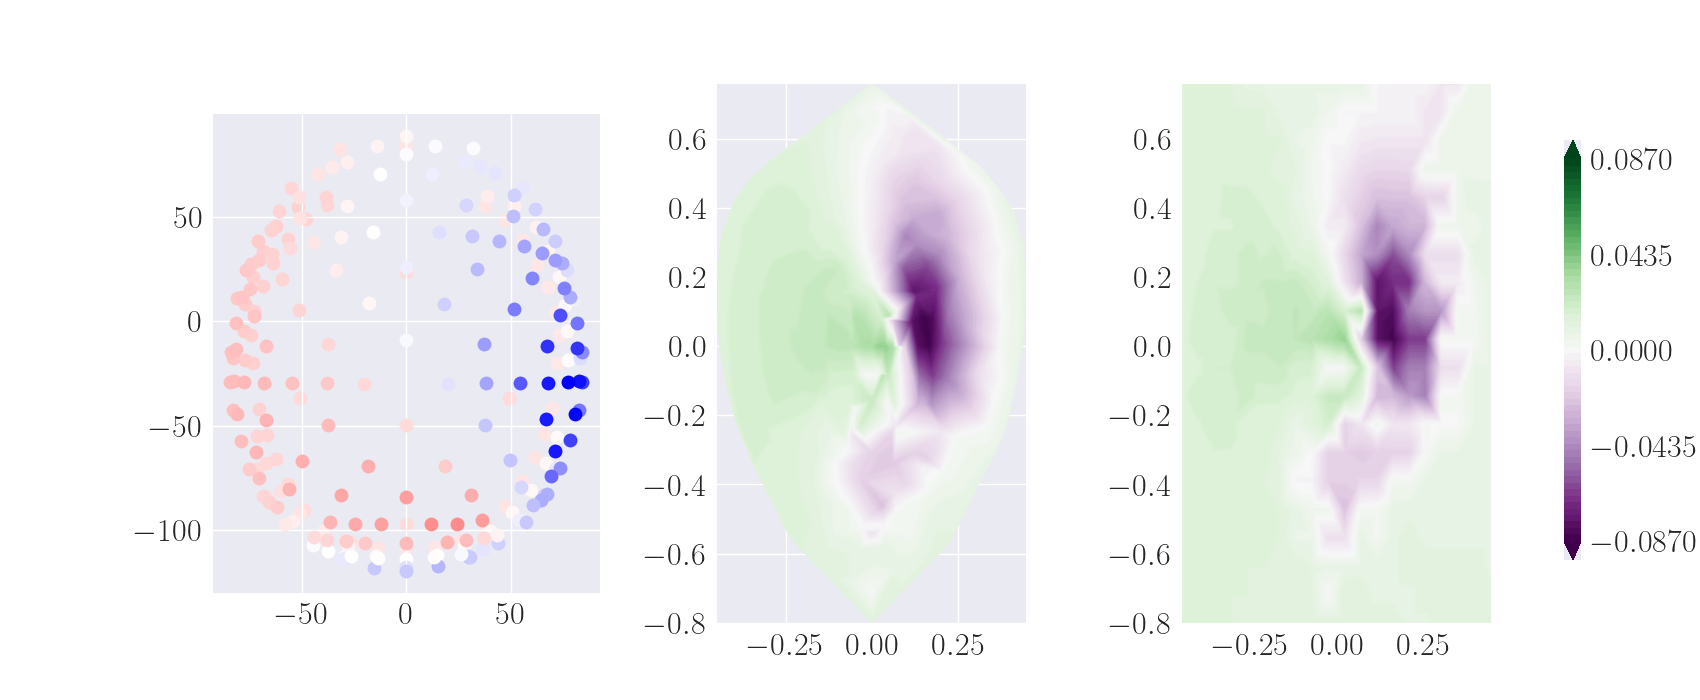
\includegraphics[width=\linewidth]{../Code/plots/finals/new_eeg_dipole_pos_4.png}
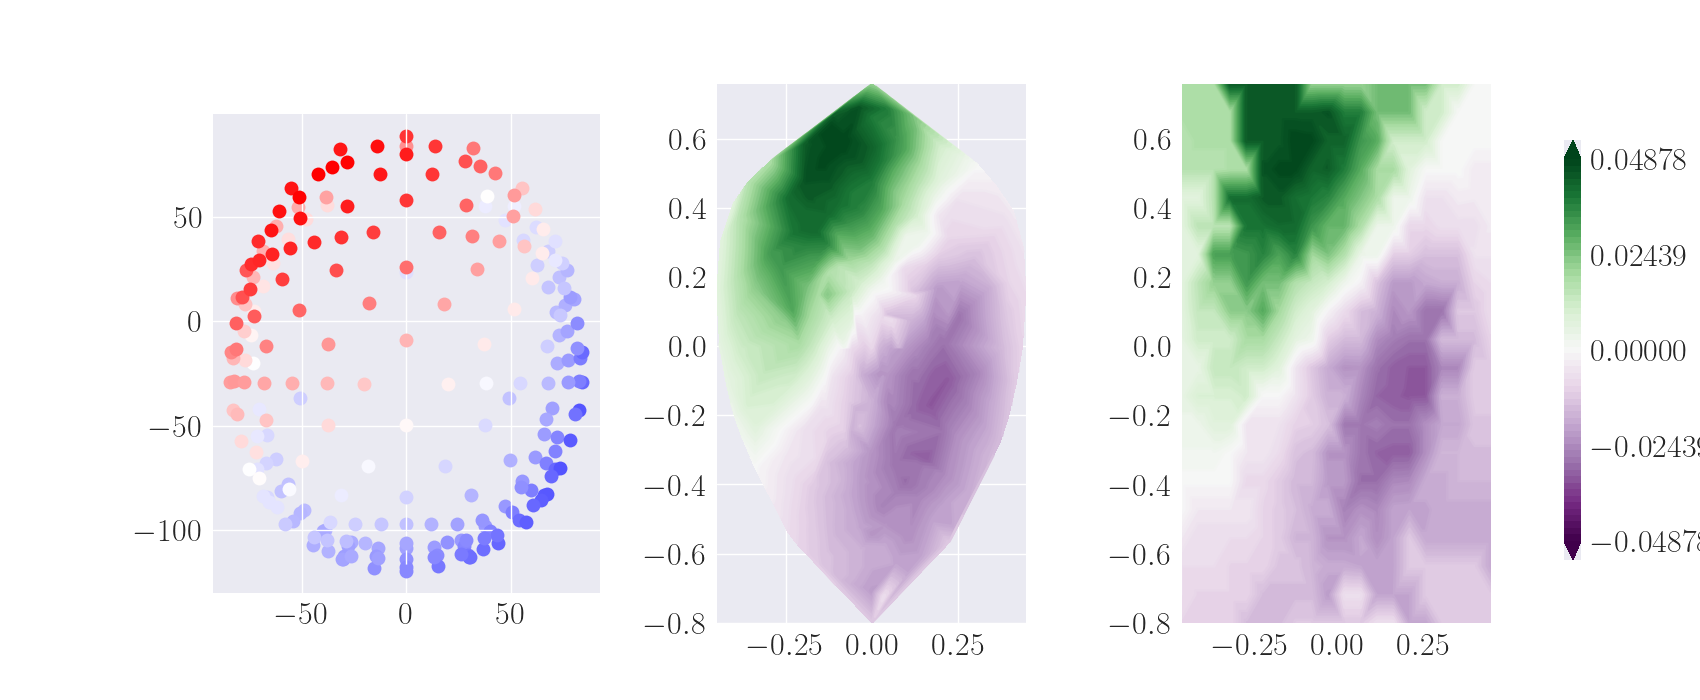
\includegraphics[width=\linewidth]{../Code/plots/finals/new_eeg_dipole_pos_6.png}

\caption{\newline
\textbf{Right}: EEG measure for 3 different samples measured in $\mu V$. \newline
\textbf{Middle and Left}: Illustration of the interpolation of the EEG data into two-dimensional matrix.}
\label{fig:eeg_dipole_pos_0}

\end{figure}

\begin{figure}[!htb]
    \centering
    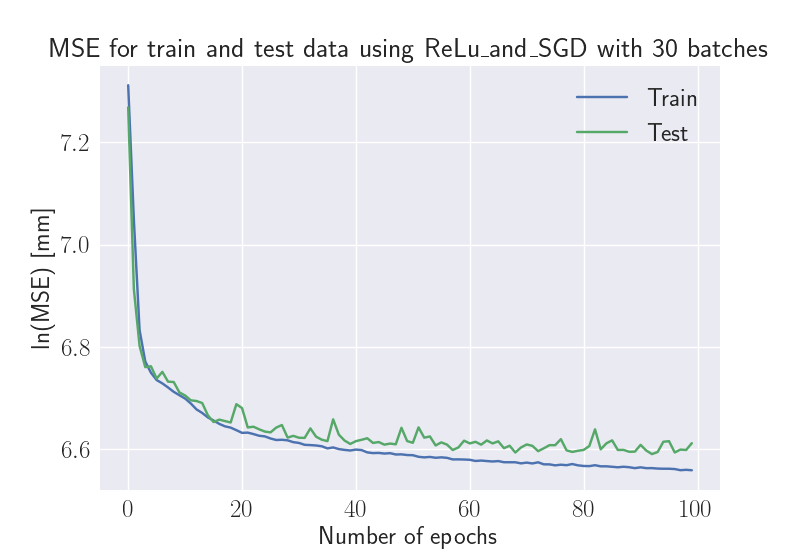
\includegraphics[width=\linewidth]{../Code/plots/finals/MSE_CNN_dipoles_2_interpolated_CNN_20x20_10000_ReLu_and_SGD_30_100.png}
    \caption{The validation accuracy for Convolutional Neural Network with 10 000 samples (20x20 matrix) with ReLU activation function. }
    \label{fig:single_dipole_accuracy_CNN_2d}
\end{figure}

% \begin{figure}[!htb]
%     \centering
%     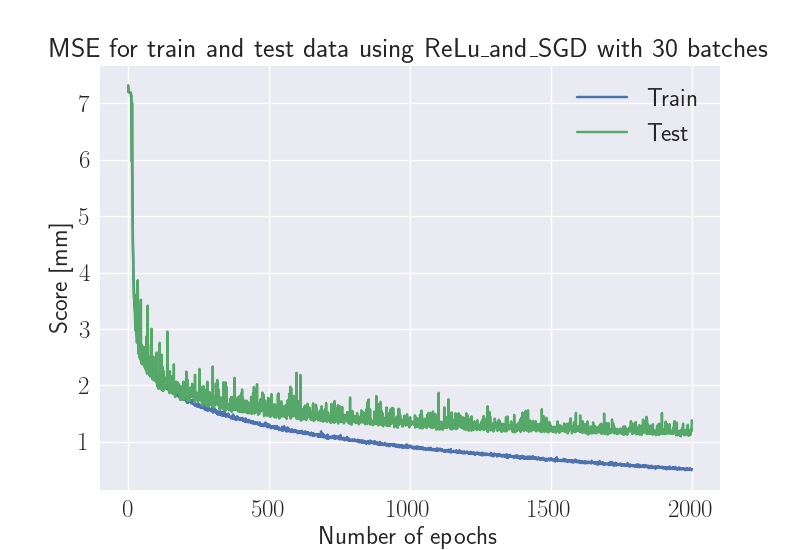
\includegraphics[width=\linewidth]{../Code/plots/CNN/MSE_interpolated_CNN_20x20_10000_ReLu_and_SGD_30_2000.png}
%     \caption{The validation accuracy for Convolutional Neural Network with 10 000 samples (20x20 interpolated matrix) with ReLU activation function. }
%     \label{fig:single_dipole_accuracy_CNN}
% \end{figure}


\section{Region of Active Correlated Current Dipoles}

Some results for the prediction of the size and location of current dipole populations.

\begin{figure}[!htb]
    \centering
    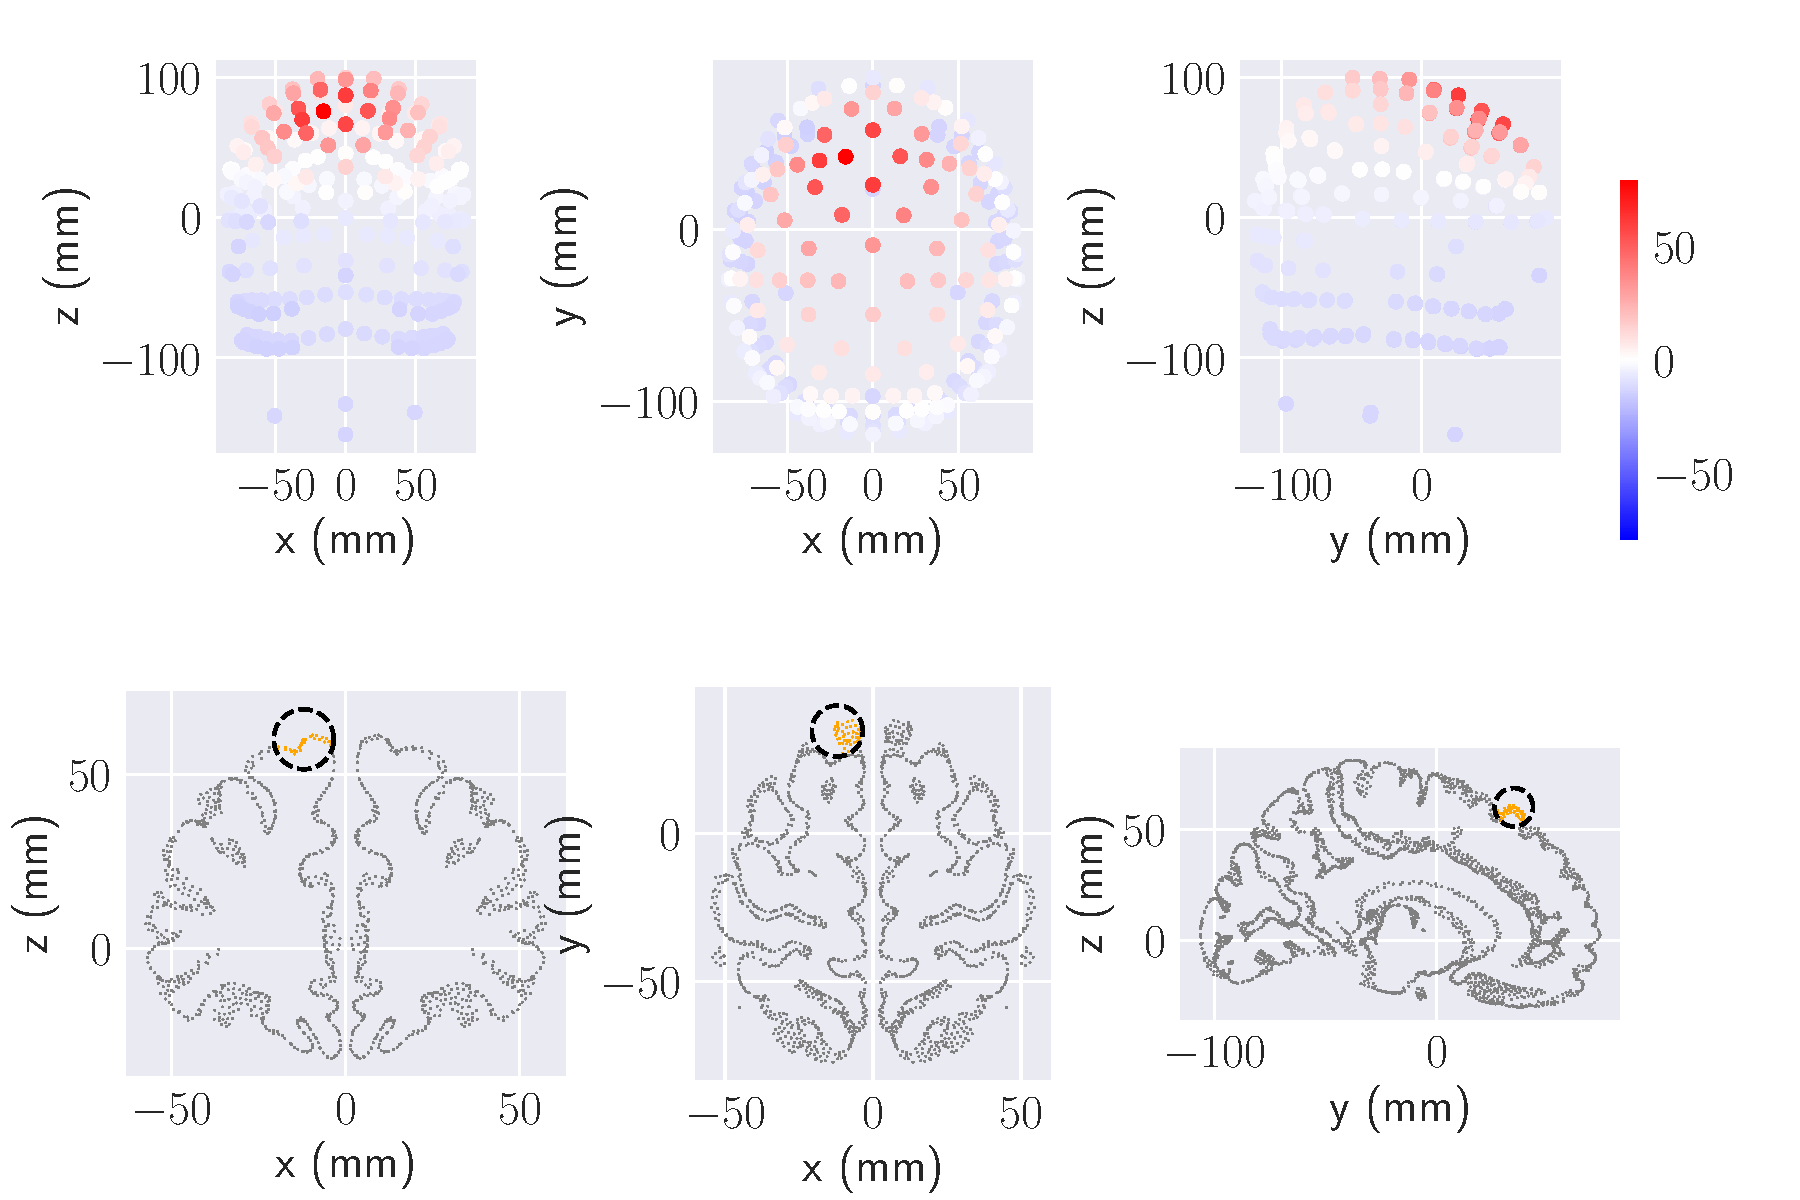
\includegraphics[width=\linewidth]{../Code/plots/finals/new_dipole_area_reduced_0.pdf}
    \caption{EEG for a sample containing a spherical population of current dipole sources with a random center within the celebral cortex. The EEG measure is seen from both sides (x-, z-plane and y-, z-plane) and above (the x-, y-plane). EEG electrode locations are presented as filled circels, where the color of the fill represents the amplitude of the measured signal for the given electrode.}
    \label{fig:dipole_area}
\end{figure}

\begin{figure}[!htb]
    \centering
    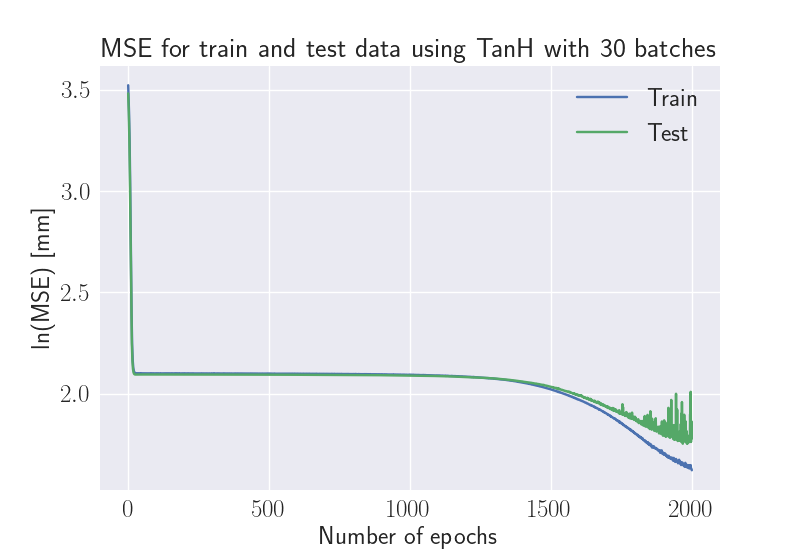
\includegraphics[width=\linewidth]{../Code/plots/finals/normalized_dipole_area.png}
    \caption{The validation accuracy for the simple Feed Forward Neural Network, predicting both center and radius for 10 000 samples, for 2000 epochs, with a learning rate equal to 0.0001.}
    \label{fig:dipole_area_result}
\end{figure}

\begin{figure}[!htb]
    \centering
    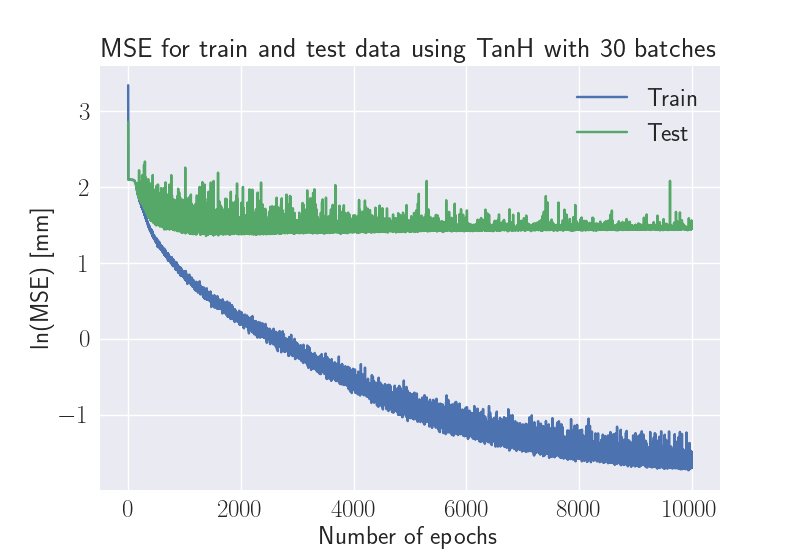
\includegraphics[width=\linewidth]{../Code/plots/finals/MSE_dipole_area_lr0.001_l1_20mm_TanH_30_10000.png}
    \caption{The validation accuracy for the simple Feed Forward Neural Network, predicting both center and radius for 10 000 samples, for 10000 epochs, with a learning rate equal to 0.001.}
    \label{fig:dipole_area_result}
\end{figure}


Printed in terminal:

Epoch 9898/9999 | Train:  0.187 | Test:  4.275

Epoch 9899/9999 | Train:  0.184 | Test:  4.288

Epoch 9900/9999 | Train:  0.201 | Test:  4.279


Target: tensor([-1.0800, -1.9594,  0.4290, 11.0140])

Predicted: tensor([-1.1171, -1.9642,  0.4575, 16.5920])


Target: tensor([-6.7642e-02,  1.5426e+00, -1.0356e-02,  1.5576e+01])

Predicted: tensor([-0.3908,  1.4285, -0.1167, 15.9222])


Target: tensor([-0.6671, -1.0569,  1.8694,  7.1385])

Predicted: tensor([-0.7248, -1.0950,  1.9903,  6.2405])



\section{Localizing Multiple Dipole Sources}
\begin{figure}[!htb]
    \centering
    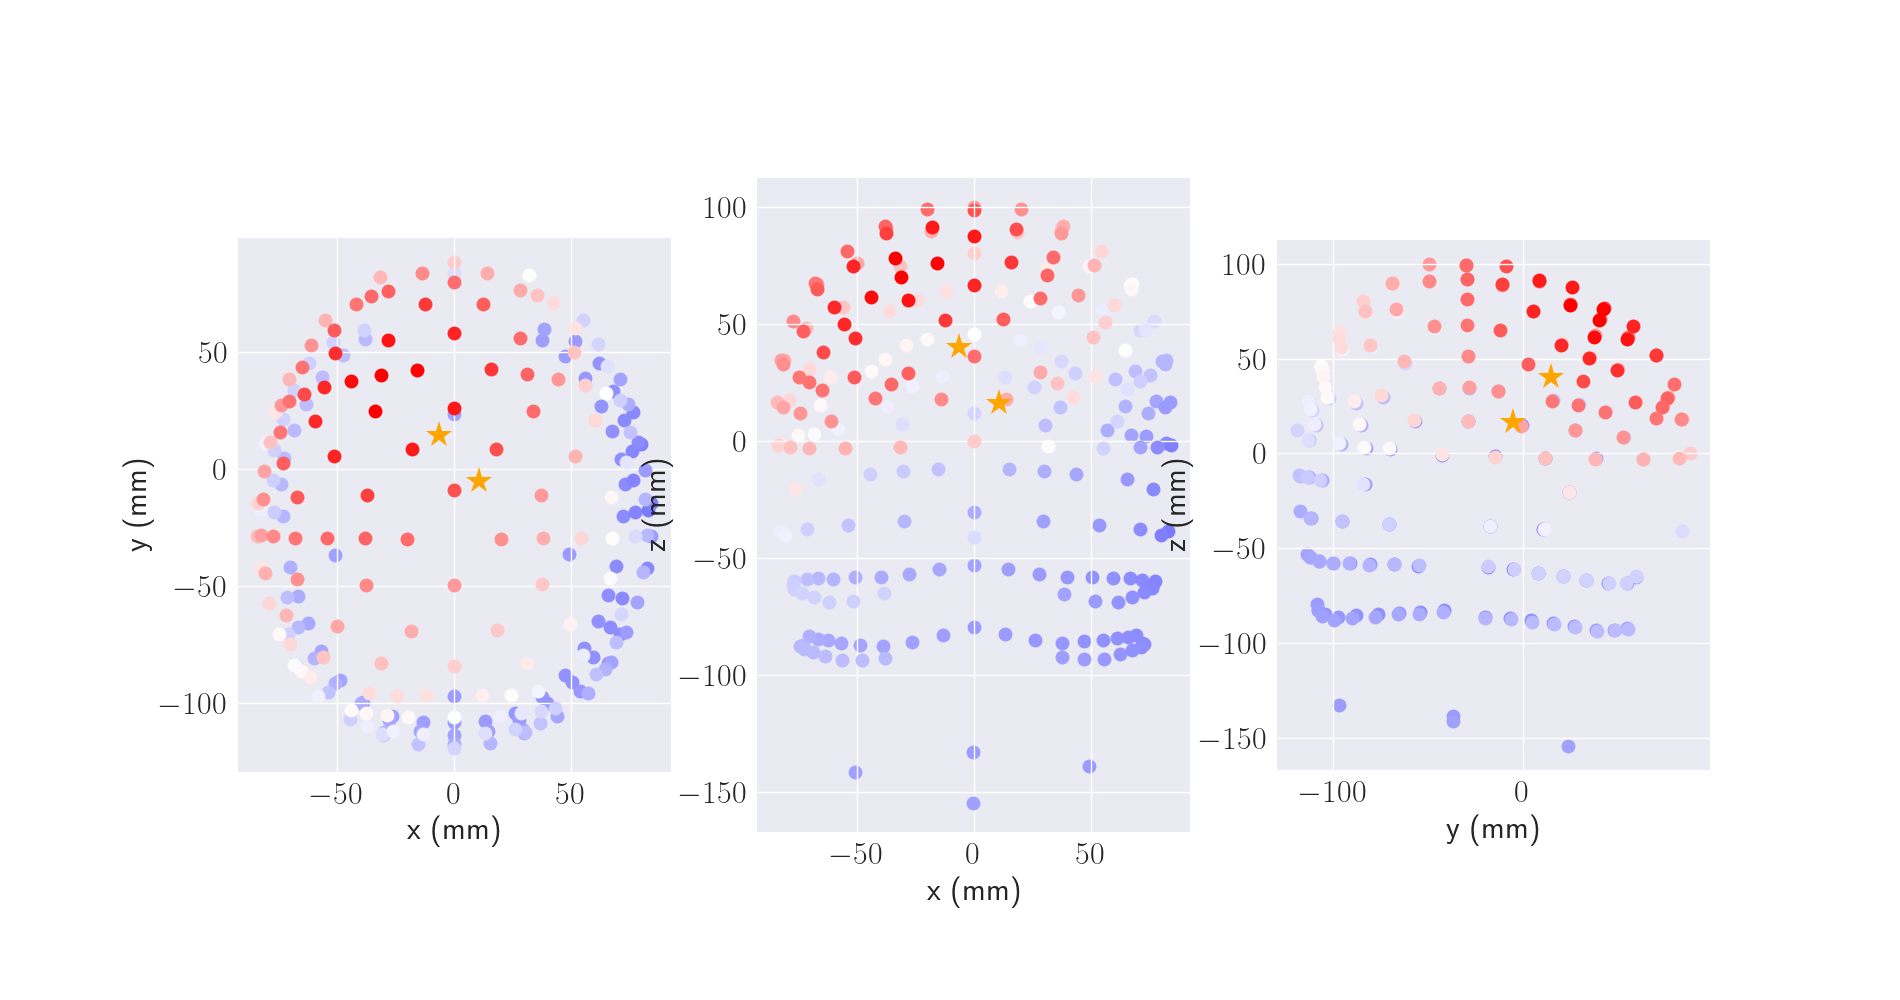
\includegraphics[width=\linewidth]{../Code/plots/finals/eeg_field_2_2.png}
    \caption{EEG for a sample containing two current dipole sources at random positions within the celebral cortex. The EEG measure is seen from both sides (x-, z-plane and y-, z-plane) and above (the x-, y-plane). EEG electrode locations are presented as filled circels, where the color of the fill represents the amplitude of the measured signal for the given electrode. The positions of the current dipole moments are marked with yellow stars.}
    \label{fig:dipole_area_result}
\end{figure}

\begin{figure}[!htb]
    \centering
    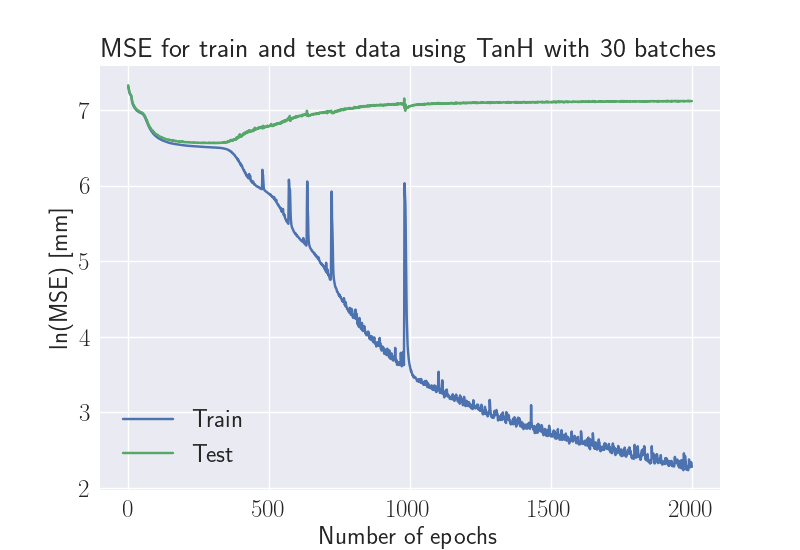
\includegraphics[width=\linewidth]{../Code/plots/finals/MSE_NN_2_10000_l1_TanH_30_2000.png}
    \caption{The validation accuracy for the simple Feed Forward Neural Network, predicting two current dipole sources.}
    \label{fig:dipole_area_result}
\end{figure}

\end{document}